\documentclass[aspectratio=169]{beamer}

\usepackage{amsmath}
\usepackage{amssymb}
\usepackage{amsfonts}
\usepackage{ytableau}
\usepackage{setspace}
\usepackage{listings}
\usepackage{graphicx}
\graphicspath{{./figures/}}
\usepackage{caption}
\usepackage{subcaption}
\usepackage{float}
% \usepackage{enumitem}
% \usepackage[p,osf]{cochineal}
% \usepackage[scale=.95,type1]{cabin}
% \usepackage[cochineal,bigdelims,cmintegrals,vvarbb]{newtxmath}
% \usepackage[zerostyle=c,scaled=.94]{newtxtt}
% \usepackage[cal=boondoxo]{mathalfa}

%Hello there
% \usetheme{metropolis}
% \setsansfont[BoldFont={Fira Sans}]{Fira Sans Light}
% \setmonofont{Fira Mono}
% \usepackage[sfdefault]{Fira Sans}
\setbeamertemplate{navigation symbols}{}
\useinnertheme{rectangles}

\newcommand{\act}[1]{%
    \begin{frame}
    \centering
    \Huge

    {\color{purple} #1}
    \end{frame}
}

\title{Limiting Shapes of Random Young Diagrams}
\newcommand{\norm}[1]{\left\lVert#1\right\rVert}
\newcommand{\cond}[2]{\mathrm{cond}_#1(#2)}
%

% \newtheorem{theorem}{Theorem}[chapter]
\newtheorem{lem}[theorem]{Lemma}
\newtheorem{defn}[theorem]{Definition}
\newtheorem{conj}[theorem]{Conjecture}
\newcommand{\perm}[1]{\left\langle#1\right\rangle}
\newcommand{\E}{\mathbb{E}}
\renewcommand{\Pr}[1]{\mathbb{P}\left(#1\right)}
\newcommand{\R}{\mathbb{R}}
\newcommand{\C}{\mathbb{C}}
\newcommand{\N}{\mathbb{N}}
\newcommand{\size}{\mathrm{size}}
\newcommand{\shape}{\mathrm{shape}}
\setstretch{1.5}
% Hello there


\begin{document}
\author{Mriganka Basu Roy Chowdhury \vskip 10pt \emph{advised by} \vskip 10pt Dr. Subhamay Saha 
%\vskip 5pt \emph{and} \vskip 5pt Prof. Manjunath Krishnapur
}
\date{Friday, 20th November, 2020}
\lstset{language=matlab}
\maketitle

\def\arraystretch{1.8}
\begin{frame}
    \frametitle{Outline of the talk}
    \begin{itemize}
        \item I will first describe a few facts about Young Tableaux.
        \item Then I will speak about the Limit Shape Theorem.
        \item Finally I will recall some basic Representation Theory and describe the problem we wish to solve.
    \end{itemize}

\end{frame}

\act{Young Diagrams}

\begin{frame}
    We begin by looking at Young Diagrams. \pause A Young Diagram is just a visual representation of a partition $p_1 \geq p_2 \geq \ldots \geq p_k \geq 1 $ of a number $p_1 + p_2 + \cdots + p_k = n \in \N$. \pause
\vskip 10pt
For example, for $n = 12$, suppose we consider a partition $12 = \perm{4 + 3 + 3 + 2}$. \pause Its Young Diagram is:
\begin{figure}
    \centering
\ydiagram{4, 3, 3, 2}
\end{figure}
\pause For any $n$, we define $YD_n := \{T \mid T \text{ is a Young Diagram of size $n$}\}$, where $\size(T) = n$ if $T$ represents a partition of $n$.
\end{frame}


\begin{frame}

    If we fill a Young Diagram with \emph{distinct} numbers from $\{1, 2, \ldots, n\} =: [n]$, such that each row and column is increasing, we call it a Standard Young Tableaux (SYT). \pause For the above diagram, this is a valid SYT:

\begin{figure}
    \centering
    \begin{ytableau}
        12 & 10 & 7 & 3\\
        11 & 9 & 5 \\
        8 & 6 & 2 \\
        4 & 1
    \end{ytableau}
\end{figure}

For any $T$, we write $SYT_T$ to be the set of all SYTs of ``shape'' $T$. And for any $n$, we write $SYT_n = \bigcup_{T \in YD_n} SYT_T$.
\end{frame}

\begin{frame}
    For any permutation $\pi$ of $[n]$, there is a way to associate a pair of SYTs with it. This is the content of the celebrated RSK Correspondence:\pause

    \begin{theorem}[RSK Correspondence]
        There is a bijection $RS$ from $S_n$ to the set of all pairs of SYTs $(P, Q)$ of same shape.
    \end{theorem}
\pause
This result is not just an existence result. There is an explicit algorithm that does this, called the \emph{Schensted Algorithm}. \pause As an example, if $\pi = \perm{4, 1, 5, 3, 2}  $, then the associated pair is:

\begin{center}
    $P = $ \begin{ytableau}
        1 & 2 \\
        3 & 5 \\
        4
    \end{ytableau}\ \ and $Q = $
    \begin{ytableau}
        1 & 3\\
        2 & 4\\
        5
    \end{ytableau}
\end{center}

\end{frame}

\begin{frame}
We now note an important consequence of the result. \pause
If $t_T = |SYT_T|$ is the number of SYTs of a given shape $T \in YD_n$, then clearly, $n! = \sum_{T \in YD_n} t^2_T$.\pause 
\vskip 10pt
This is an extremely important fact in the Representation Theory of the Symmetric Group $S_n$ (more later). \pause It can also be seen from a Markov Chain Structure on the set of all Young Diagrams, called the \emph{Bratelli Diagram}. This last idea is outlined in the report, but we do not go into this here.
\end{frame}

\begin{frame}
    But perhaps more importantly, $RS$ can be used to define a natural measure on the set of all Young Diagrams of size $n$. \pause

    \begin{defn}[Plancherel Measure]
        Let $\pi \in S_n$ be uniformly distributed. Then $\shape(RS(\pi)) = \lambda$ is an random element in $YD_n$. The distribution of $\lambda$ is called the Plancherel Measure on $YD_n$. From the above discussion, 
        \[ p_T = t^2_T / n! \]
    where $p_T$ is the probability of $T$ under the Plancherel Measure.
    \end{defn}\pause
    Note that, $\shape(RS(\pi))$ is the shape of either of the two SYTs produced (which is unambiguous because they have the same shape).\vskip 10pt

\end{frame}

\act{The Limit Shape Theorem}

\begin{frame}
Now, suppose we take a Plancherel Distributed $\lambda \in YD_n$, for large $n$. Equivalently, we take a uniformly distributed $\pi \in S_n$, and take the shape of the 
diagrams formed under $RSK$. \emph{What does it look like?} \vskip 10pt \pause
In the following, we do not draw Young Diagrams as above.
Instead, we rotate it by $135^{\circ}$ and scale everything appropriately (for reasons that will be clear):

\begin{figure}
    \centering
    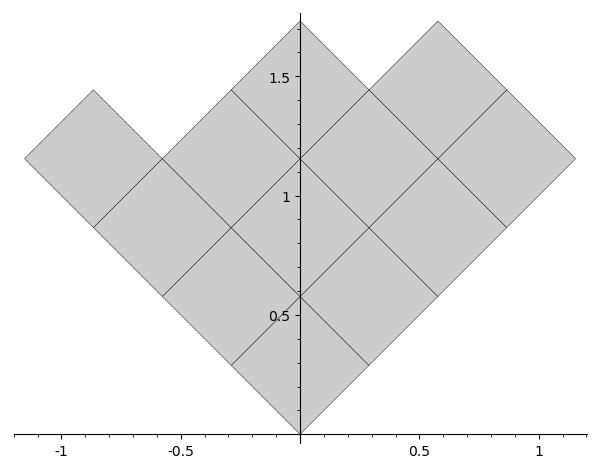
\includegraphics[width=0.35\textwidth]{simpyd}
\end{figure}

\end{frame}

\begin{frame}\begin{figure}
    \centering
    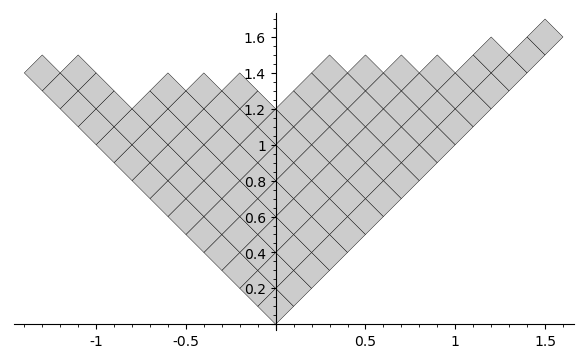
\includegraphics[width = 0.8\textwidth]{pic100}
    \caption{$n = 100$}
\end{figure}
\end{frame}

\begin{frame}
\begin{figure}
    \centering
    \centering
    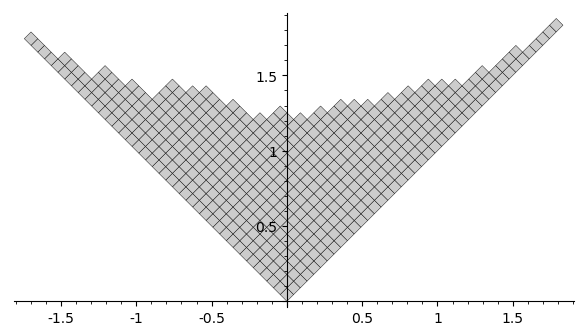
\includegraphics[width = 0.8\textwidth]{pic500}
\caption{$n = 500$}\end{figure}
\end{frame}

\begin{frame}
\begin{figure}
    \centering
    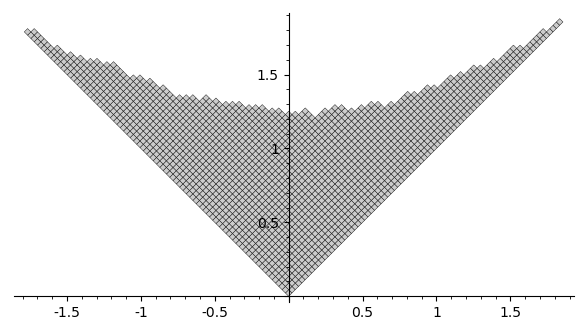
\includegraphics[width = 0.8\textwidth]{pic2000}
\caption{$n = 2000$}\end{figure}
\end{frame}


\begin{frame}
\begin{figure}
    \centering
    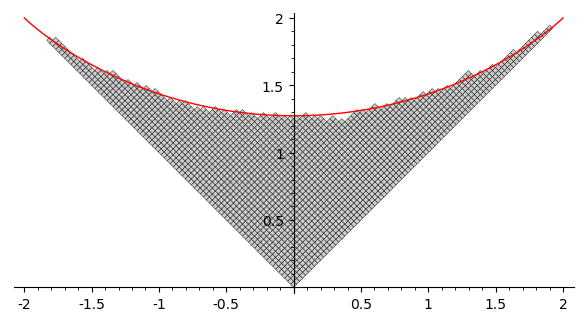
\includegraphics[width = 0.8\textwidth]{pic2000sur}
\caption{$n = 2000$ again}\end{figure}
\end{frame}

\begin{frame}
    This limit shape is the content of the celebrated Logan-Shepp-Vershik-Kerov result. \pause
    \begin{theorem}[Logan-Shepp-Vershik-Kerov, 1977]
        Under appropriate scaling, and with an appropriate metric on the space of all 1-Lipschitz compactly supported functions with area $2$ between the graph of the function and $y = |x|$ (see the report for details), the function corresponding to a Plancherel-random Young Diagram converges to 
    \begin{equation*}
        \Omega(u) =%
        \begin{cases}
            \dfrac{2}{\pi}\left(u \sin^{-1}\left(\dfrac{u}{2}\right) + \sqrt{4 - u^2}\right) & |u| \leq 2\\
            |u| & |u| > 2\\   
        \end{cases}
    \end{equation*}
    which is the {\color{red} red} line above.
    \end{theorem}
\end{frame}

\act{Some Representation Theory}

\begin{frame}
    We now revisit some basic Representation Theory. Note that all our groups are finite, and all our vector spaces are finite dimensional. 
    \begin{itemize}
        \item<2-> A representation of a group $G$ on a vector space $V$ is a homomorphism $G \to GL(V)$, where $GL(V)$ is the space of all invertible linear maps $V \to V$. 
        \item<3-> Two representations $\phi : G \to GL(V)$, $\psi : G \to GL(W)$ are \emph{equivalent} if there exists an invertible map $T : V \to W$ such that $T^{-1}\psi(g)T = \phi(g)$ for all $g \in G$.
        \item<4-> Every representation is equivalent to a representation $\rho : G \to GL(\C^n)$ on $\C^n$ for some $n$, such that $\rho(g)$ is unitary for all $g \in G$. Such a representation is called \emph{unitary}.
        \item<5-> For a given group $G$, there are only finitely many distinct irreducible (defined later) representations upto equivalence. 
    \end{itemize}
\end{frame}

\begin{frame}
    \begin{itemize}
        \item<1-> Given two representations $\phi : G \to GL(V), \psi : G \to GL(W)$, there is a representation $\phi \oplus \psi : G \to GL(V \oplus W)$, called the \emph{direct sum}, defined by \[(\phi \oplus \psi)(g)(v \oplus w) = (\phi(g)(v)) \oplus (\psi(g)(w))\]
        \item<2-> Also, with the above notation, there is a representation $\phi \otimes \psi : G \to GL(V \otimes W)$, called the \emph{tensor product}, defined by \[(\phi \otimes \psi)(g)(v \otimes w) = (\phi(g)(v)) \otimes (\psi(g)(w))\] and extended by linearity.
    \end{itemize}
\end{frame}

\begin{frame}
    \begin{itemize}
            \item<1-> A unitary representation $\rho : G \to GL(V)$ is called irreducible if there is no subspace $W \subsetneq V, W \neq \{0\}$, such that $\rho(g)W \subseteq W$ for all $g \in G$.
            \item<2-> Given any representation $\rho$, it is possible find finitely many irreducible representations $\psi_1, \psi_2, \ldots, \psi_k$ such that \[ \rho \sim \psi_1 \oplus \psi_2 \oplus \psi_3 \oplus \cdots \oplus \psi_k\]
    where $\sim$ denotes equivalence.
    \end{itemize}
\end{frame}


\begin{frame}
    \begin{itemize}
        \item<1-> It can be shown that for the symmetric group $S_n$, each irreducible representation corresponds to a Young Diagram of size $n$.
        \item<2-> Thus, given $T \in YD_n$, we write $[T]$ for the irreducible representation corresponding to $T$.
    \end{itemize}
\end{frame}

\act{Transition Measures}


\begin{frame}
    We need to introduce another object before we can proceed further. \pause Given a Young Diagram, we can associate a measure to it, called the Transition Measure. \pause First, we rotate the diagram as above. Consider $16 = \perm{5 + 3 + 3 + 2 + 2 + 1}$. It has the diagram:\pause
    \begin{figure}
        \centering
        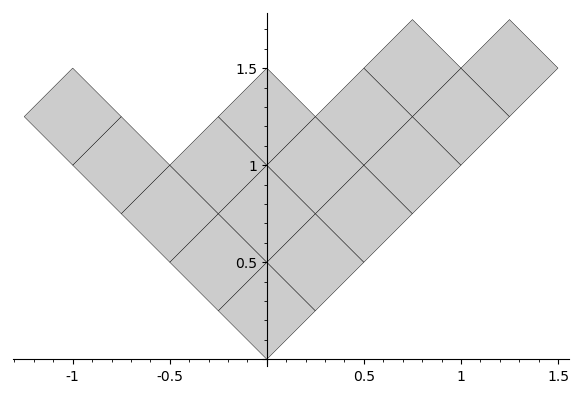
\includegraphics[width = 0.3\textwidth]{trans1}
    \end{figure}\pause
    and consider the ``interlacing'' sequence $x_1 < y_1 < x_2 < \ldots < y_{k - 1} < x_k$ of minima and maxima.
\end{frame}

\begin{frame}
    Associate to each $x_i$ a probability of $p_i = \dfrac{t_{T'}}{\size(T')t_T}$ where $T'$ is the YD obtained by adding a cell to the minima. \pause It can be proved that $\sum{t_{T'}} = (n + 1)\size(T)$, where the sum is over all Young Diagrams that can be obtained from $T$ by adding a boundary cell, and $n = \size(T)$. \pause So $p_i$ form a probability measure on $\R$. The following shows the transition measure for the above diagram. \pause
    \begin{figure}
        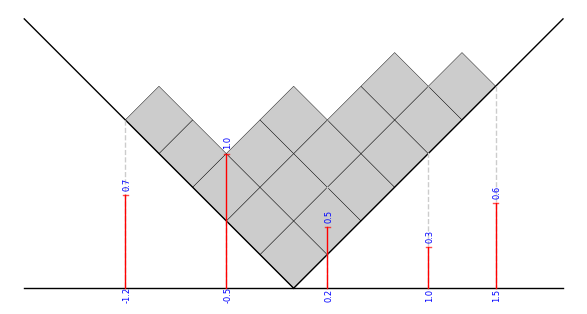
\includegraphics[width = 0.45\textwidth]{trans2}
        \caption{The transition measure. Here we report $q_k = p_k / \max p_k$.}
    \end{figure}
\end{frame}


\act{Now we can look at our problem}

\begin{frame}
    There is noncommutative analog of the classical convolution of measures, called the \emph{free convolution}. \pause However, to describe it, we need to develop the ideas of Non-commutative Probability, which is done in the report. \pause
    \vskip 10pt \noindent Here we only mention an example of free convolution that we will need later. Consider $\mu = \frac{1}{2}(\delta_1 + \delta_{-1})$. Then, $\mu \boxplus \mu = \text{arcsine}[-2, 2]$. \pause This fact is derived from first principles in the report. 
    \vskip 10pt \noindent However, notice the difference between this and the classical convolution. In the classical case, we would have $\frac{1}{4}(\delta_{2} + 2\delta_0 + \delta_{-2})$, which is a discrete measure. \pause But the free convolution gives us a continuous measure.
\end{frame}

\newcommand{\biane}{\mathrm{BianeComb}}
\begin{frame}
    In 1998, Biane considered the following operation on two Young Tableaux: \pause


\begin{defn}[Biane's combination]
    Given two Young Diagrams $T, T' \in YD_n$, consider the corresponding representations $[T], [T']$ of $S_n$. We define Biane's combination as:
    \[%
        \biane(T, T') = \{S \in YD \mid [S] \text{ is an irreducible component of } [T] \otimes [T']\}
    \]
\end{defn}
\end{frame}

\begin{frame}
Under some technical conditions, he proved:

\begin{theorem}
    Given two Young Diagrams $T, T' \in YD_n$, a large fraction of the elements $\lambda$ of $\biane(T, T')$ satisfies:
    \[%
        \mu_T \boxplus \mu_T' \approx \mu_\lambda \text{ as $n \to \infty$}
    \]
    where $\mu_T$ is the transition measure associated with $T$, for some appropriate meaning of $\approx$. 
\end{theorem}
\end{frame}

\begin{frame}
We consider the following shuffle: \pause

\begin{defn}[Alternate Shuffle]
    Given two Young Diagrams $T, T' \in YD_n$, define the random Young Diagram $\lambda = \lambda_{T, T'}$ as follows:
    \[%
        \lambda = \shape(RS(\mathrm{Shuffle}(\pi, \pi')))
    \]
    where $\pi$ and $\pi'$ are uniformly random permutations with $\shape(RS(\pi)) = T$ and $\shape(RS(\pi')) = T'$ respectively. \pause Also $\mathrm{Shuffle}(\pi \in S_n, \pi' \in S_m) = \tau$ is a random variable defined as follows: let $S \subseteq [n + m]$ be a uniformly random subset of size $n$. Then $\tau \in S_{n + m}$ has the positions in $S$ filled by $\pi$ (in order), and the positions in $[n + m] - S$ filled by $\pi' + n$. 
\end{defn}


\end{frame}


\begin{frame}
 
Uniformly random permutations $\pi$ with $\shape(RS(\pi)) = T$ can be generated as follows: \pause
\begin{enumerate}
    \item<2-> Generate two independent SYT $P, Q \in SYT_n$, with $\shape(P) = \shape(Q) = T$, uniformly. 
    \item<3-> Construct $\pi = RS^{-1}(P, Q)$.
\end{enumerate}

\pause
The step for generating uniform SYT with given shape is nontrivial. The celebrated Greene-Nijenhuis-Wilf algorithm does this via an elegant ``hook walk'' procedure.
\end{frame}


\begin{frame}
Consider $T = T' = \perm{m^2 = m + m + \ldots + m}$, with the following diagram for $m = 20$: \pause
\begin{center}
    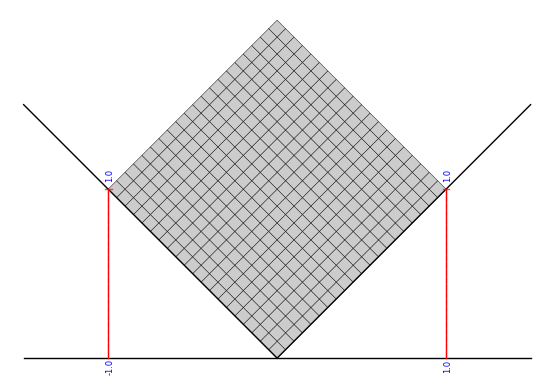
\includegraphics[width=0.5\textwidth]{sqyd}
\end{center}

with the transition measure $\tau = \frac{1}{2}\left(\delta_{-1} + \delta_{1}\right)$
\end{frame}

\begin{frame}

After doing the Alternate Shuffle above (and averaging over several iterations), we get the following Young Diagram: \pause
\begin{center}
    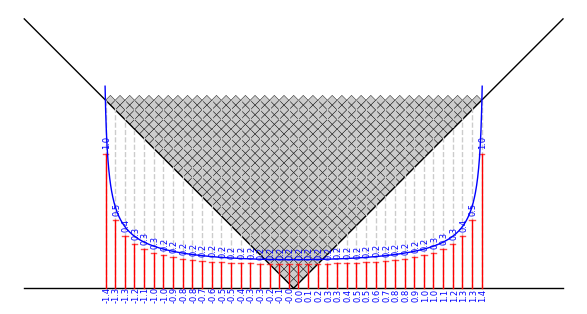
\includegraphics[width=0.6\textwidth]{shuffle}
\end{center}
\pause
As we can see, there is significant match between the computed transition measure, and the $arcsine$ distribution, plotted in {\color{blue} blue}.

\end{frame}

\begin{frame}
    Inspired from this, we formulate the following conjecture:



\begin{conj}
    The ``typical'' transition measure of the Alternate Shuffle of two Young Diagrams with transition measures $\mu$ and $\nu$ is the free convolution $\mu \boxplus \nu$ of the two transition measures (upto scaling along the real line).
\end{conj}
\pause Of course, we will need to precisely define ``typical''. But right now, our primary focus is to understand related constructions, and thinking about how we can handle such objects better.
\end{frame}

\act{Thank You}
\act{Intuition for the Free Convolution}

\newcommand{\weak}{\stackrel{w}{\longrightarrow}}

\begin{frame}
    Given a Symmetric real matrix $A$, let $\lambda_1 \geq \lambda_2 \geq \ldots \geq \lambda_n$ be its eigenvalues. \pause We write,

    \[ \mu_A = \frac{1}{n}\sum_{i = 1}^{n} \delta_{\lambda_i} \in \mathcal{P}(\R)\]

    for the \emph{Empirical Spectral Distribution} (ESD) of $A$. This is a fundamental object of study in Random Matrix Theory. \pause If we have a family of matrices $A_n$, we say that it has the $\mu$ as the \emph{limiting} ESD if $\mu_A \weak \mu$. \vskip 10pt \pause
    Now, suppose $A_n, B_n$ are two families of matrices such that $\mu_{A_n} \weak \mu$ and $\mu_{B_n} \weak \nu$. \pause Then consider the random matrices $C_n := Q^T_nA_nQ_n, D_n := S^TB_nS$, where $Q_n, S_n$ are independent families of uniform orthogonal matrices of size $n$. \pause Clearly, $A_n$ and $C_n$ have the same ESD, and similarly for $B_n$ and $D_n$. 
\end{frame}

\begin{frame}
    The question now is, \emph{what is the limiting ESD for} $C_n + D_n$ ? That is, given two ``typical'' random matrices with given limiting ESD, what is the limiting ESD for their sum? \pause Let us look at a simulation: Let $A_n = \text{diag}(\underbrace{-1, -1, -1, \ldots, -1}_{\text{$n$ $-1$s}}, \underbrace{1, 1, \ldots, 1}_{\text{$n$ $1$s}})$, and let $B_n = A_n$. \pause Then, clearly, $\mu_{A_n} = \frac{1}{2}(\delta_1 + \delta_{-1}) = \mu_{B_n}$ which is also their limiting ESD. \pause Here is a picture of the ESD for $C_n + D_n$ where $n = 1000$
\end{frame}


\begin{frame}
\begin{figure}
    \centering
    \centering
    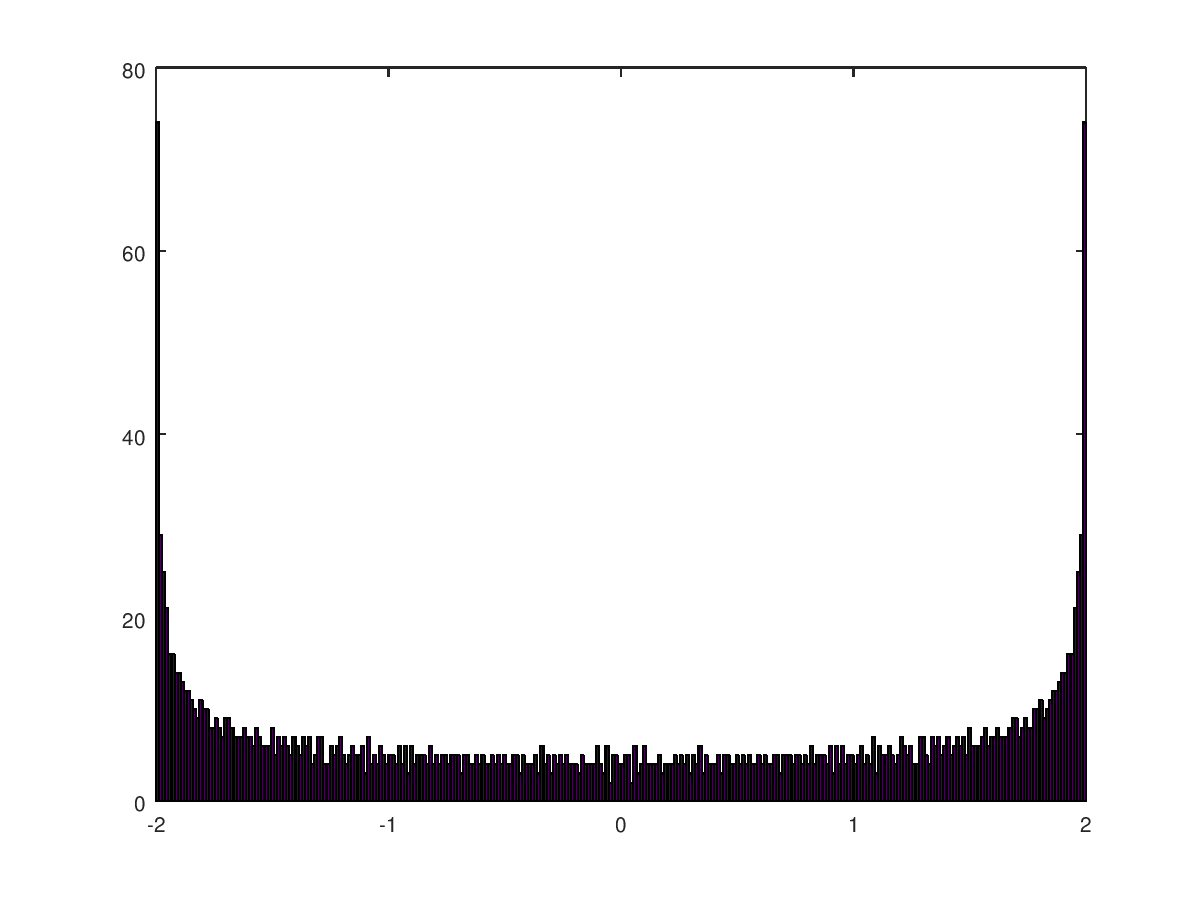
\includegraphics[width = 0.5\textwidth]{freeconv}
    \caption{ESD for $C_n + D_n$, $n = 1000$}
\end{figure}

As we can see, this is very close to the $\text{arcsine}[-2, 2]$ distribution, which was seen to be the free convolution of $\frac{1}{2}(\delta_{1} + \delta_{-1})$ with itself. 
\end{frame}

\begin{frame}
    This is indeed a general theorem. The limiting ESD for $C_n + D_n = \mu \boxplus \nu$. \pause Of course, we need to interpret the limit in a suitable sense. In most cases, it is a limit in probability, with a metric which metrizes the weak topology on $\mathcal{P}(\R)$. \vskip 10pt \noindent
    This is the intuition for the free convolution. The non-commutativity arises in some sense from the noncommutativity of the matrices.
\end{frame}

\end{document}
